\documentclass[10pt,a4paper]{article}
\usepackage[margin=2cm]{geometry}
\usepackage{amsmath,amssymb}
\usepackage{graphicx,booktabs,xcolor,array,makecell,tikz}
\usepackage{listings}
\usepackage[colorlinks=true,linkcolor=blue!50!black,urlcolor=blue!50!black]{hyperref}
\usepackage{microtype}

\lstset{language=Python,basicstyle=\ttfamily\small,keywordstyle=\color{blue!60!black}\bfseries,
  commentstyle=\color{green!40!black},stringstyle=\color{red!50!black},
  frame=single,framerule=0.3pt,rulecolor=\color{gray!60},backgroundcolor=\color{gray!5},
  columns=fullflexible,keepspaces=true,showstringspaces=false,
  numbers=left,numberstyle=\tiny\color{gray},xleftmargin=1.5em,aboveskip=6pt,belowskip=4pt}
\newcommand{\code}[1]{\texttt{#1}}
\newcommand{\Pp}{\mathcal P}\newcommand{\Qq}{\mathcal Q}
\newcommand{\curl}{\operatorname{curl}}\renewcommand{\div}{\operatorname{div}}
\setlength{\parindent}{0pt}\setlength{\parskip}{4pt}\setlength{\emergencystretch}{3em}\sloppy

% dof tables
\definecolor{gr}{RGB}{0,140,60}\definecolor{bl}{RGB}{30,70,200}
\newcommand{\G}[1]{\textcolor{gr}{\textbf{#1}}}\newcommand{\B}[1]{\textcolor{bl}{\textbf{#1}}}
\newcommand{\tot}[1]{\\[1pt]$=$\,\textbf{#1}}
\newcommand{\cc}[1]{\makecell[l]{#1}}
\tikzset{wf/.style={thick},hd/.style={thin,dashed}}
\newcommand{\trigic}{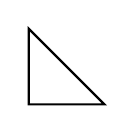
\begin{tikzpicture}[scale=0.8]\draw[wf](0,0)--(1.2,0)--(0,1.2)--cycle;\end{tikzpicture}}
\newcommand{\quadic}{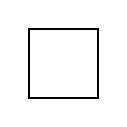
\begin{tikzpicture}[scale=0.8]\draw[wf](0,0)rectangle(1.1,1.1);\end{tikzpicture}}
\newcommand{\tetic}{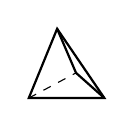
\begin{tikzpicture}[scale=0.8]\coordinate(A)at(0,0);\coordinate(B)at(1.2,0);\coordinate(C)at(0.75,0.4);\coordinate(D)at(0.45,1.1);
 \draw[wf](A)--(B)--(D)--cycle;\draw[wf](B)--(C)--(D);\draw[hd](A)--(C);\end{tikzpicture}}
\newcommand{\prismic}{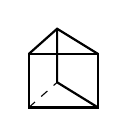
\begin{tikzpicture}[scale=0.8]\coordinate(A)at(0,0);\coordinate(B)at(1.1,0);\coordinate(C)at(0.45,0.4);
 \coordinate(D)at(0,0.85);\coordinate(E)at(1.1,0.85);\coordinate(F)at(0.45,1.25);
 \draw[wf](A)--(B)--(E)--(D)--cycle;\draw[wf](D)--(F)--(E);\draw[wf](B)--(C)--(F);\draw[hd](A)--(C);\end{tikzpicture}}
\newcommand{\hexic}{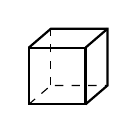
\begin{tikzpicture}[scale=0.8]\draw[wf](0,0)rectangle(0.9,0.9);\draw[wf](0.9,0)--(1.25,0.3)--(1.25,1.2)--(0.35,1.2)--(0,0.9);\draw[wf](0.9,0.9)--(1.25,1.2);
 \draw[hd](0,0)--(0.35,0.3)--(1.25,0.3);\draw[hd](0.35,0.3)--(0.35,1.2);\end{tikzpicture}}

\title{\vspace{-1.2cm}High-Order de Rham Sequences on Mixed Meshes in NGSolve\\[2pt]
\large The spaces \code{H1}, \code{HCurl}, \code{HDiv}, \code{L2}: orders, flags and degrees of freedom}
\author{Joachim Sch\"oberl}
\date{NGSolve Technical Note 2026-01\quad\textbullet\quad November 2026}

\begin{document}
\maketitle\vspace{-0.9cm}

\section{Conventions}

The finite element spaces \code{H1}, \code{HCurl}, \code{HDiv} and \code{L2} of NGSolve form exact sequences
\[
  H^1 \xrightarrow{\ \nabla\ } H(\curl) \xrightarrow{\ \curl\ } H(\div) \xrightarrow{\ \div\ } L^2
\]
on triangles, quadrilaterals, tetrahedra, prisms and hexahedra, and on meshes that mix these shapes.
One order convention holds for all shapes: the order $k$ is the polynomial degree of the trace, $\Pp_k$ on edges and triangular faces, $\Qq_k$ on quadrilateral faces. Since the traces do not depend on the element shape or on the flags below, all variants are conforming to each other.

\begin{itemize}\setlength\itemsep{1pt}
\item \code{H1(k)}: $\Pp_k$ on simplices, $\Qq_k$ on quads and hexes, $\Pp_k(x,y)\otimes\Pp_k(z)$ on prisms. \code{L2(k)} uses the same polynomials without continuity.
\item \code{HCurl(k)} $= \nabla\,$\code{H1(k+1)} $\oplus\, Z_k$. The tangential trace has degree $k$. The non-gradient part $Z_k$ has injective curl, and $\curl Z_k$ lies in \code{HDiv(k-1)}. With \code{type1=True} only the gradients of \code{H1(k)} are used; $Z_k$ stays the same. Thus \code{type1} removes the top-degree gradients, and the edge traces drop to degree $k-1$.
\item \code{HDiv(k)}: the normal trace has degree $k$. The space consists of facet functions, divergence-free cell bubbles $B_k$, and a cell part $D_q$ with $\div D_q = $ \code{L2(q)}$/\mathbb R$. With \code{RT=True}, $q=k$ and $\div$ maps onto \code{L2(k)}; with \code{RT=False}, $q=k-1$. Thus \code{RT} adds the top-degree divergences. If \code{RT} is not given, quads, prisms and hexes use \code{RT=True}, and trigs, tets and pyramids use \code{RT=False}.
\end{itemize}
Below, \code{HCurl(k,type1)}, \code{HDiv(k,RT)} and \code{HDiv(k,BDM)} are short for \code{type1=True}, \code{RT=True} and \code{RT=False}.
The spaces are nested,
\[
\text{\code{HCurl(k,type1)}} \subset \text{\code{HCurl(k)}} \subset \text{\code{HCurl(k+1,type1)}},\qquad
\text{\code{HDiv(k,BDM)}} \subset \text{\code{HDiv(k,RT)}} \subset \text{\code{HDiv(k+1,BDM)}},
\]
and they contain the full polynomials $\Pp_k^d \subset$ \code{HCurl(k)}, $\Pp_{k-1}^d\subset$ \code{HCurl(k,type1)}, $\Pp_k^d\subset$ \code{HDiv(k,BDM)}.
On simplices these are the classical elements: \code{HCurl(k,type1)} and \code{HCurl(k)} are the N\'ed\'elec elements of the first \cite{ned80} and second kind \cite{ned86}, \code{HDiv(k,RT)} and \code{HDiv(k,BDM)} the Raviart--Thomas and Brezzi--Douglas--Marini elements.

The basis functions are hierarchical and follow the construction of \cite{zaglmayr,sz05}: each space consists of lowest-order functions, of the images of the high-order functions of the previous space, and of functions that complete the space. This splitting holds separately on every edge, face and cell (local complete sequence property). It is the reason why gradients or divergences can be switched on and off by flags, and it is shown in the tables of Section 3.

\section{Exact sequences}

For every choice of the two flags the spaces fit together. In three dimensions the sequences
\begin{align*}
\text{(A)}\quad & \text{\code{H1(k)}} \xrightarrow{\nabla} \text{\code{HCurl(k,type1)}} \xrightarrow{\curl} \text{\code{HDiv(k-1,RT)}} \xrightarrow{\div} \text{\code{L2(k-1)}}\\
\text{(B)}\quad & \text{\code{H1(k)}} \xrightarrow{\nabla} \text{\code{HCurl(k,type1)}} \xrightarrow{\curl} \text{\code{HDiv(k-1,BDM)}} \xrightarrow{\div} \text{\code{L2(k-2)}}\\
\text{(C)}\quad & \text{\code{H1(k+1)}} \xrightarrow{\nabla} \text{\code{HCurl(k)}} \xrightarrow{\curl} \text{\code{HDiv(k-1,RT)}} \xrightarrow{\div} \text{\code{L2(k-1)}}\\
\text{(D)}\quad & \text{\code{H1(k+1)}} \xrightarrow{\nabla} \text{\code{HCurl(k)}} \xrightarrow{\curl} \text{\code{HDiv(k-1,BDM)}} \xrightarrow{\div} \text{\code{L2(k-2)}}
\end{align*}
are exact on contractible domains: the range of each operator is the kernel of the next one, and $\div$ is onto. On tetrahedra these are the four sequences of Arnold, Falk and Winther \cite{afw06}; (A) is the sequence of the first kind, (D) of the second kind. The same four sequences exist on prisms, hexes and mixed meshes.
In two dimensions the sequences are \code{H1(k)} $\to$ \code{HCurl(k,type1)} $\to$ \code{L2(k-1)} and \code{H1(k+1)} $\to$ \code{HCurl(k)} $\to$ \code{L2(k-1)}. The 2D \code{HDiv} spaces are the rotated \code{HCurl} spaces, \code{HDiv(k,BDM)} $=$ rot \code{HCurl(k)} and \code{HDiv(k,RT)} $=$ rot \code{HCurl(k+1,type1)}.

If \code{RT} is not given, the divergence maps onto \code{L2(k-1)} on quads, prisms and hexes, and onto \code{L2(k-2)} on trigs and tets. The space \code{V.CreateDivergenceSpace()} is the \code{L2} space with these element-wise orders, so that
\[
\text{\code{H1(k+1)}} \xrightarrow{\nabla} \text{\code{HCurl(k)}} \xrightarrow{\curl} \text{\code{V = HDiv(k-1)}} \xrightarrow{\div} \text{\code{V.CreateDivergenceSpace()}}
\]
is exact on mixed meshes as well, also with \code{HCurl(k,type1)} and \code{H1(k)} in front.

\section{Degrees of freedom}

The tables show the element spaces of the sequences that start from \code{H1(2)}, with the number of dofs per vertex (V), edge (E), triangular face (T), quadrilateral face (Q) and cell (C), and the element dimension. Black is the lowest-order dof (Whitney edge function, RT$_0$ face function), \G{green} dofs span the kernel of the outgoing operator (gradients in \code{HCurl}, divergence-free functions in \code{HDiv}), \B{blue} dofs are mapped injectively into the next space. The green dofs of one space are the images of the blue dofs of the previous one, node by node.

\begin{center}\small
\renewcommand{\arraystretch}{1.1}
\begin{tabular}{@{}c|c|cc|cc@{}}\toprule
 & \code{H1(2)} & \code{HCurl(2,type1)} & \code{HCurl(1)} & \code{L2(1)} & \code{L2(0)}\\\midrule
\raisebox{-5mm}{\trigic} &
\cc{V: 1\\E: 1\tot{6}} &
\cc{E: 1+\G1\\C: \B2\tot{8}} &
\cc{E: 1+\G1\tot{6}} &
\cc{$\Pp_1$\tot{3}} & \cc{$\Pp_0$\tot{1}}\\
 & $\Pp_2$ & N\'ed\'elec 1st kind $=$ rot RT$_1$ & N\'ed\'elec 2nd kind $=\Pp_1^2$ & & \\\midrule
\raisebox{-6mm}{\quadic} &
\cc{V: 1\\E: 1\\C: 1\tot{9}} &
\cc{E: 1+\G1\\C: \G1+\B3\tot{12}} &
\cc{E: 1+\G1\\C: \G1\tot{9}} &
\cc{$\Qq_1$\tot{4}} & \cc{$\Qq_0$\tot{1}}\\
 & $\Qq_2$ & $N_{[1]}=\Qq_{1,2}\times\Qq_{2,1}$ & $\nabla\Qq_2+N_{[0]}$ & & \\\bottomrule
\end{tabular}
\end{center}

On the quad, \code{HCurl(k,type1)} is the tensor-product N\'ed\'elec space $N_{[k-1]}=\Qq_{k-1,k}\times\Qq_{k,k-1}$. The default space \code{HCurl(k)} $=\nabla\Qq_{k+1}+N_{[k-1]}$ has dimension $(k{+}2)^2-1+k^2$; its curl is $\Qq_{k-1}$, as $\Pp_{k-1}$ on the triangle. The cell dofs of order $k$ are
\begin{center}\small
\begin{tabular}{@{}l@{\qquad}l@{\qquad}l@{}}
 & \code{HCurl(k)} & \code{HCurl(k,type1)}\\[2pt]
trig & \G{$\dfrac{k(k-1)}2$} $+$ \B{$\dfrac{(k+2)(k-1)}2$} & \G{$\dfrac{(k-1)(k-2)}2$} $+$ \B{$\dfrac{(k+2)(k-1)}2$}\\[7pt]
quad & \G{$k^2$} $+$ \B{$k^2-1$} & \G{$(k-1)^2$} $+$ \B{$k^2-1$}
\end{tabular}
\end{center}

\begin{center}\small
\setlength{\tabcolsep}{4.5pt}\renewcommand{\arraystretch}{1.1}
\begin{tabular}{@{}c|c|cc|ccc|cc@{}}\toprule
 & \code{H1(2)} & \code{HCurl(2,type1)} & \code{HCurl(1)} & \code{HDiv(1,RT)} & \code{HDiv(1,BDM)} & \code{HDiv(0)} & \code{L2(1)} & \code{L2(0)}\\\midrule
\raisebox{-5mm}{\tetic} &
\cc{V: 1\\E: 1\tot{10}} &
\cc{E: 1+\G1\\T: \B2\tot{20}} &
\cc{E: 1+\G1\tot{12}} &
\cc{T: 1+\G2\\C: \B3\tot{15}} &
\cc{T: 1+\G2\tot{12}} &
\cc{T: 1\tot{4}} &
\cc{$\Pp_1$\tot{4}} & \cc{$\Pp_0$\tot{1}}\\\midrule
\raisebox{-7mm}{\prismic} &
\cc{V: 1\\E: 1\\Q: 1\tot{18}} &
\cc{E: 1+\G1\\T: \B2\\Q: \G1+\B3\\C: \B2\tot{36}} &
\cc{E: 1+\G1\\Q: \G1\tot{21}} &
\cc{T: 1+\G2\\Q: 1+\G3\\C: \G2+\B5\tot{25}} &
\cc{T: 1+\G2\\Q: 1+\G3\\C: \G2\tot{20}} &
\cc{T,Q: 1\tot{5}} &
\cc{$\Pp_1\!\otimes\!\Pp_1$\tot{6}} & \cc{\tot{1}}\\\midrule
\raisebox{-7mm}{\hexic} &
\cc{V: 1\\E: 1\\Q: 1\\C: 1\tot{27}} &
\cc{E: 1+\G1\\Q: \G1+\B3\\C: \G1+\B5\tot{54}} &
\cc{E: 1+\G1\\Q: \G1\\C: \G1\tot{31}} &
\cc{Q: 1+\G3\\C: \G5+\B7\tot{36}} &
\cc{Q: 1+\G3\\C: \G5\tot{29}} &
\cc{Q: 1\tot{6}} &
\cc{$\Qq_1$\tot{8}} & \cc{$\Qq_0$\tot{1}}\\\bottomrule
\end{tabular}
\end{center}

The alternating sum of the element dimensions is 1 for each sequence, for example (A) on the prism: $18-36+25-6=1$, and (C) on the hex: $27-31+6-1=1$.
The face dofs of the 3D elements are those of the 2D elements: a quadrilateral face of \code{HCurl(2,type1)} carries \G1+\B3 dofs like the cell of the quad, a triangular face \B2. This makes meshes of tets, prisms and hexes conforming.
The cell dofs show the bubble spaces: the blue cell dofs of \code{HCurl} and the green cell dofs of \code{HDiv} both count the divergence-free bubbles $B_1$ (tet 0, prism 2, hex 5), and the blue cell dofs of \code{HDiv} count $\dim$\code{L2}$\,-\,1$.

\paragraph{Element spaces.}
The following table lists the spaces for general order. \code{HCurl(k)} is \code{HCurl(k,type1)} plus the gradients of \code{H1(k+1)} on every shape.
\begin{center}\small
\renewcommand{\arraystretch}{1.15}
\begin{tabular}{@{}l>{\raggedright}p{7.0cm}>{\raggedright\arraybackslash}p{8.0cm}@{}}\toprule
 & \code{HCurl(k,type1)} & \code{HDiv(k,RT)}\\\midrule
tet & N\'ed\'elec first kind, $\Pp_{k-1}^3 + x\times\tilde\Pp_{k-1}^3$ & Raviart--Thomas, $\Pp_k^3+x\,\tilde\Pp_k$\\
hex & $N_{[k-1]} = \Qq_{k-1,k,k}\times\Qq_{k,k-1,k}\times\Qq_{k,k,k-1}$ & RT$_{[k]}=\Qq_{k+1,k,k}\times\Qq_{k,k+1,k}\times\Qq_{k,k,k+1}$\\
prism & $N^{\triangle}_k\otimes\Pp_k(z)$ horizontal, $\Pp_k(x,y)\otimes\Pp_{k-1}(z)$ vertical & RT$^{\triangle}_k\otimes\Pp_k(z)$ horizontal, $\Pp_k(x,y)\otimes\Pp_{k+1}(z)$ vertical\\\bottomrule
\end{tabular}
\end{center}
Here $\tilde\Pp_k$ are the homogeneous polynomials, and $N^\triangle_k$, RT$^\triangle_k$ are the triangle spaces \code{HCurl(k,type1)} and \code{HDiv(k,RT)}.
\code{HDiv(k,BDM)} is the subspace of \code{HDiv(k,RT)} with divergence in \code{L2(k-1)}; on tets it is $\Pp_k^3$.
Element dimensions for $k=1,2,3$:
\begin{center}\small
\begin{tabular}{@{}lccccc@{}}\toprule
 & \code{H1(k)}, \code{L2(k)} & \code{HCurl(k,type1)} & \code{HCurl(k)} & \code{HDiv(k,BDM)} & \code{HDiv(k,RT)}\\\midrule
trig  & 3, 6, 10  & 3, 8, 15   & 6, 12, 20   & 6, 12, 20   & 8, 15, 24\\
quad  & 4, 9, 16  & 4, 12, 24  & 9, 19, 33   & 9, 19, 33   & 12, 24, 40\\
tet   & 4, 10, 20 & 6, 20, 45  & 12, 30, 60  & 12, 30, 60  & 15, 36, 70\\
prism & 6, 18, 40 & 9, 36, 90  & 21, 58, 125 & 20, 57, 124 & 25, 69, 146\\
hex   & 8, 27, 64 & 12, 54, 144& 31, 91, 205 & 29, 89, 203 & 36, 108, 240\\\bottomrule
\end{tabular}
\end{center}

\section{Flags and helper functions}

\begin{center}\small
\renewcommand{\arraystretch}{1.15}
\begin{tabular}{@{}>{\raggedright}p{6.4cm}>{\raggedright\arraybackslash}p{9.8cm}@{}}\toprule
\code{HCurl(mesh, order=k, type1=True)} & gradients of \code{H1(k)} instead of \code{H1(k+1)}, on all shapes\\
\code{HDiv(mesh, order=k, RT=True)}, \code{RT=False} & the same choice on all shapes\\
\code{trigRT}, \code{quadRT}, \code{tetRT}, \code{prismRT}, \code{hexRT}, \code{pyramidRT} & choice per element shape, overrides \code{RT}, e.g.\ \code{HDiv(mesh, order=2, RT=False, hexRT=True)}\\
\code{hodivfree=True} & facet functions and $B_k$ only; the divergence is piecewise constant\\
\code{order=0} & RT$_0$ on all shapes, independent of \code{RT}\\\bottomrule
\end{tabular}
\end{center}
The flags change only cell dofs of \code{HDiv} and only gradient dofs of \code{HCurl}, so every combination is conforming. \code{HDivSurface} takes the same \code{RT} flags.

\code{V.CreateDivergenceSpace()} returns the \code{L2} space onto which $\div$ maps \code{V}: order $k$ on elements with \code{RT}, order $k-1$ on the others, and order $0$ with \code{hodivfree}. On a mixed mesh with default flags neither \code{L2(mesh, order=k)} nor \code{L2(mesh, order=k-1)} is the right pressure space for \code{HDiv(mesh, order=k)}; the first is too large on simplices, the second too small on tensor-product elements.
\code{G, W0 = W1.CreateGradient()} returns the matching space \code{W0}, which is \code{H1(k+1)} or with \code{type1} \code{H1(k)}, and the sparse matrix \code{G} of the embedding $\nabla:$ \code{W0} $\to$ \code{W1}.

\paragraph{Example.}
The script builds the default sequence on an hp-refined mesh of the Fichera corner, which consists of 501 tets, 209 prisms and 37 hexes.
\begin{lstlisting}
from ngsolve import *
from netgen.occ import *

# hp-refined Fichera corner: tets, prisms and hexes
cube = Box((0,0,0), (2,2,2))
cube.edges.hpref = 1
geo = OCCGeometry(Box((-1,-1,-1), (1,1,1)) - cube)
mesh = Mesh(geo.GenerateMesh(maxh=0.4))
mesh.RefineHP(levels=2, factor=0.2)

k = 2
W0 = H1(mesh, order=k+1)
W1 = HCurl(mesh, order=k)            # or HCurl(mesh, order=k+1, type1=True)
W2 = HDiv(mesh, order=k-1)           # RT on prisms/hexes, BDM on tets
W3 = W2.CreateDivergenceSpace()      # L2(k-1) there, L2(k-2) on tets
nd = [W.FreeDofs().NumSet() for W in (W0, W1, W2, W3)]   # used dofs
print(nd, nd[0] - nd[1] + nd[2] - nd[3])

# curl of an HCurl function is represented exactly in HDiv
u = GridFunction(W1)
u.Set(CF((sin(y*z), x*z, exp(x)*y)))
w = GridFunction(W2)
w.Set(curl(u))
print(sqrt(Integrate((w - curl(u))**2, mesh)))
print(sqrt(Integrate(div(w)**2, mesh)))
\end{lstlisting}
It prints the dimensions \code{[7363, 13261, 7950, 2051]} with alternating sum 1, the Euler characteristic of the domain, and the errors $7\cdot10^{-15}$ and $2\cdot10^{-13}$. The count uses \code{FreeDofs} instead of \code{ndof}, since \code{RefineHP} leaves unused edges and faces in the mesh, and their dofs are contained in \code{ndof}.

\section{Verification and limits}

\paragraph{Tests.}
Exactness was tested algebraically, by comparing the ranks of the operators with the space dimensions and by checking that the $L^2$-projection of $\nabla u$, $\curl u$, $\div u$ onto the next space reproduces it.
\begin{itemize}\setlength\itemsep{1pt}
\item Mesh of one hex, two prisms and two tets, with two vertex numberings: sequences (A)--(D) and the default sequences with \code{CreateDivergenceSpace} are exact for $k\le 3$.
\item Mesh of 12 trigs and 10 quads: both \code{HCurl} sequences, and \code{H1(k+1)} $\to$ \code{HDiv(k)} $\to$ divergence space for \code{RT} set, unset and \code{False}, are exact for $k\le4$.
\item The inclusions of the full polynomials and the nesting of the spaces of Section 1 hold on the mixed 3D mesh for $k\le 3$ and $k \le 2$, respectively. The dof counts of Section 3 are those reported by the spaces.
\end{itemize}

\paragraph{Changes against version 6.2.2604.}
Triangles and tets are unchanged. On quads, prisms and hexes the default \code{HCurl(k)} is smaller: the curl now has degree $k-1$ as on simplices (quad \code{HCurl(1)}: 12 $\to$ 9 dofs, prism 30 $\to$ 21, hex 54 $\to$ 31). On quads and hexes the former space is available as \code{HCurl(k+1,type1)}.
\code{type1} on prisms and hexes was a mixture of both kinds whose curl kernel was larger than $\nabla\,$\code{H1(k)}; \code{HCurl(2,type1)} went from 67 to 36 dofs on the prism and from 132 to 54 on the hex.
The \code{HDiv} prism is now the tensor-product Raviart--Thomas space (\code{HDiv(1)}: 27 $\to$ 25 dofs). \code{RT=False} was ignored on quads, prisms and hexes and now selects the smaller space.

\paragraph{Limits.}
\begin{itemize}\setlength\itemsep{1pt}
\item Pyramids are conforming to all neighbours, and $\ker\curl=\nabla H^1$ holds. For \code{HCurl} of order $k\ge2$ the curl is not contained in \code{HDiv(k-1)} on pyramids, so sequences on meshes with pyramids are exact only at lowest order.
\item On non-affine quads and hexes the stages $\nabla$ and, in 3D, $\curl$ stay exact. The last operator maps into $J^{-1}\,$\code{L2} instead of \code{L2}, where $J$ is the Jacobian determinant; the ranks of the operators are unchanged.
\item Anisotropic polynomial orders on prisms and hexes are not tested with the new spaces.
\end{itemize}

{\footnotesize\setlength{\itemsep}{0pt}
\begin{thebibliography}{9}\setlength{\itemsep}{1pt}
\bibitem{zaglmayr} S.~Zaglmayr. \emph{High Order Finite Element Methods for Electromagnetic Field Computation}. PhD thesis, Johannes Kepler University Linz, 2006.
\bibitem{sz05} J.~Sch\"oberl and S.~Zaglmayr. High order N\'ed\'elec elements with local complete sequence properties. \emph{COMPEL} 24(2):374--384, 2005.
\bibitem{afw06} D.~N.~Arnold, R.~S.~Falk and R.~Winther. Finite element exterior calculus, homological techniques, and applications. \emph{Acta Numer.} 15:1--155, 2006.
\bibitem{ned80} J.-C.~N\'ed\'elec. Mixed finite elements in $\mathbb R^3$. \emph{Numer. Math.} 35:315--341, 1980.
\bibitem{ned86} J.-C.~N\'ed\'elec. A new family of mixed finite elements in $\mathbb R^3$. \emph{Numer. Math.} 50:57--81, 1986.
\end{thebibliography}}

\end{document}
